\section{Additional Numerical Explorations}

\label{2605:app:numerical-extra}


\subsection{Neural LoFi Kernel Limit} \label{2605:app:kernel-limit}

\begin{figure}
    \centering
    
    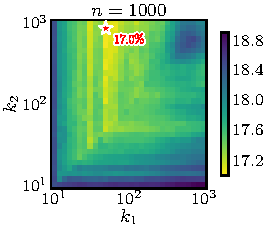
\includegraphics[width=0.32\linewidth]{figs/kernel_error_1k}
    
    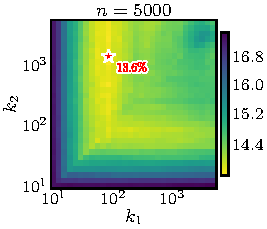
\includegraphics[width=0.32\linewidth]{figs/kernel_error_5k}
    
    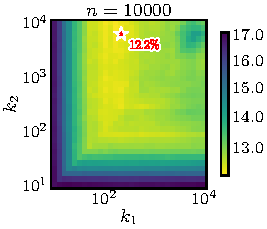
\includegraphics[width=0.32\linewidth]{figs/kernel_error_10k}
    \caption{
        Test Error (\%) as a function of the kept features for Kernel LoFi for different training dataset sizes $n$.
        Stars indicate the best $(k_1,k_2)$ in each grid. The optimal retained dimension is finite and different from the usual kernel case (upper right corner), mirroring the behavior of the finite-width Neural LoFi heatmaps in~\Cref{2605:fig:heatmaps}
    }
    \label{2605:fig:kernel-heatmaps}
\end{figure}

The kernel formulation of Neural LoFi developed in
Appendix~\ref{2605:app:kernel-nlofi} replaces the random projections $\bm R_\ell$ of
Algorithm~\ref{2605:alg:neural-lofi} by their kernel expectations and computes the
generalized eigenvalue problem of Proposition~\ref{2605:prop:generalized-eigenvector}
on the $n{\times}n$ Gram matrix. The resulting estimator is deterministic in the projection
randomness and depends on $(\bm x_{1:n}, y_{1:n})$ only through the kernel
$K_{\ell-1}$ and the labels. 

Figure~\ref{2605:fig:kernel-heatmaps} reports the test error of kernel LoFi on
binary CIFAR-10 over the per-layer retained ranks $(k_1,k_2)$, at two
training-set sizes. 
First, the error
landscape is U-shaped in the same way as its finite-width counterpart in
\Cref{2605:fig:heatmaps}: keeping too few features discards predictive signal,
keeping too many includes eigendirections that are not separated from the
noise bulk at this sample size, and the optimum sits at intermediate
$(k_1,k_2)$. 
Second, the location of this optimum shifts toward larger
ranks as $n$ grows. 
Both effects are those predicted by the
relevance--complexity criterion of Theorem~\ref{2605:thm:variational-rkhs} and
the emergence threshold of \cref{2605:eq:lofi-emergence-threshold}: more
samples lower the noise floor $\tau^k_\ell(n)$, allowing additional
low-degree directions to cross it.

Read together with the convergence experiment of
Figure~\ref{2605:fig:nlofi-convergence}, in which the finite-width LoFi error
approaches the kernel-LoFi error from above as the projection width $p$
grows, this establishes that the U-shape and the sample-dependent rank
optimum are properties of the supervised spectral mechanism itself rather
than artifacts of the random projections used in practice. 
This is also
what distinguishes kernel LoFi from standard fixed-kernel methods such as
the NNGP or NTK: the operator diagonalized at each layer is built from the
labels, so the geometry in which the next layer searches for signal changes
with the task. 
Kernel LoFi is, in this sense, the simplest deterministic
object that captures the layerwise task-adaptivity of feature learning
described in the main text.


The Neural LoFi kernel also gives a feature-space perspective on why overparameterization and pruning are not contradictory. Classical pruning methods show that many weights or connections can be removed after training with little loss in performance
\cite{lecun1989optimal,han2015learning}, while the lottery-ticket hypothesis suggests that large dense networks may contain smaller trainable subnetworks
\cite{frankle2020linear}. In Neural LoFi, width and rank play complementary roles: large width creates a rich feature space in which task-correlated directions can be discovered, while spectral pruning retains only the directions that finite data can reliably support. Thus large networks are useful for discovery, but low-rank feature selection controls the effective dimension used for prediction.



\subsection{Measuring the feature alignment of LoFi with GD} \label{2605:app:gd-feature-alignment}
In order to establish if the features learned by LoFi are a good approximation of those learned by GD, we aim to measure how the alignment grows during GD training, when compared with the features learned by LoFi. 

Let's consider a setting where we train the same architecture with both GD and LoFi, and we measure the overlap between the features at each layer. More concretely, let \(\vec{z}_{\ell}^{\text{LoFi}}(x_\mu)\) denote the features at layer \(\ell\) learned by LoFi, and let \(\vec{z}_{\ell}^{\text{GD}}(x_\mu, t)\) denote the features at the same layer learned by GD at training step \(t\); both are vector representations of the same dimension \(p_\ell\). We can then compute the \emph{featurewise overlap} as
\begin{equation}
    \left[F_{\ell}(t)\right]_{ij} = \frac{1}{n} \sum_{\mu=1}^n \frac{\left(\vec{z}_{\ell,i}^{\text{LoFi}}(x_\mu) - \left\langle\vec{z}_{\ell,i}^{\text{LoFi}}\right\rangle\right) \left(\vec{z}_{\ell,j}^{\text{GD}}(x_\mu, t) - \left\langle\vec{z}_{\ell,j}^{\text{GD}}(t)\right\rangle\right)}{\sqrt{\left(\vec{z}_{\ell,i}^{\text{LoFi}}(x_\mu) - \left\langle\vec{z}_{\ell,i}^{\text{LoFi}}\right\rangle\right)^2} \sqrt{\left(\vec{z}_{\ell,j}^{\text{GD}}(x_\mu, t) - \left\langle\vec{z}_{\ell,j}^{\text{GD}}(t)\right\rangle\right)^2}},
\end{equation}
where \(\left\langle\vec{z}_{\ell,i}^{\text{LoFi}}\right\rangle\) and \(\left\langle\vec{z}_{\ell,j}^{\text{GD}}(t)\right\rangle\) denote the mean of the respective features across the dataset. This matrix \(F_{\ell}(t)\in \mathbb{R}^{p_\ell \times p_\ell}\) captures the pairwise correlations between the features learned by LoFi and GD at layer \(\ell\) and training step \(t\). Features are permutation invariant, so we consider the \emph{Frobenius norm} of the overlap matrix as a measure of overall alignment, normalized by its initial value at random initialization:
\begin{equation}
    \text{Normalized Overlap}_{\ell}(t) = \frac{\|F_{\ell}(t)\|_F- \|F_{\ell}(0)\|_F}{\|F_{\ell}(0)\|_F}.
\end{equation}
The normalization is required because having every layer a different \(p_\ell\) and different spreadness of the features, the initial overlap at random initialization can be different across layers, and we want to measure the relative growth of the alignment during training.

In Figure~\ref{2605:fig:gradient-alignment}, we plot the evolution of \(\text{Alignment}_{\ell}(t)\) for each layer \(\ell\) during GD training, for a 4 layer fully-connected network trained on a binary classification task on CIFAR-10. 


\subsection{Generalization and Spectral Performance: GD vs. LoFi} 
\label{2605:app:gd-spectral-performance-comp}
In this experiment we aim to train networks for image binary classification (Animals vs. Vehicles in CIFAR-10) using both Neural LoFi and Gradient Descent (GD), and compare their generalization performance across a range of training set sizes. 
We investigate the generalization properties of Neural LoFi relative to GD by evaluating their test performance across varying training set sizes $n \in [10^2, 5 \times 10^4]$. To ensure a controlled comparison, we fix the architectures for both FC and CNN models to have a comparable number of parameters and identical random projection dimensions.


For GD, we employ a compute-constrained training protocol where the total number of gradient steps is held constant across dataset sizes. We adopt an adaptive scaling law for the learning rate, $\eta \propto \sqrt{B/n}$, where $B$ is the batch size, and utilize a cosine annealing schedule with a linear warmup. This ensures stable convergence dynamics without the need for exhaustive per-configuration hyperparameter tuning. In contrast, LoFi remains a one-pass algorithm requiring only the selection of the eigenvector bottleneck $k_\ell$.

Figure~\ref{2605:fig:gd-lofi-comparison} illustrates the test error as a function of the training set size. We observe that LoFi achieves generalization performance comparable to, and in low-sample regimes occasionally superior to, GD. By reporting GD performance at varying step intervals, we demonstrate that LoFi, despite being a one-pass spectral method, captures a feature set equivalent to that learned by GD during its early-to-mid training stages. 

While GD eventually outperforms LoFi as the training budget increases, this gap is expected; GD iteratively refines features across the full model capacity, whereas LoFi performs a sequential, layer-wise spectral projection. Crucially, these results are obtained without auxiliary regularization (e.g., dropout, early stopping) or optimized filtering levels for LoFi. Thus, the results in Figure~\ref{2605:fig:gd-lofi-comparison} suggest that the spectral alignment of LoFi is not merely a theoretical property but a robust driver of generalization in deep architectures.

\begin{figure}
    \centering
    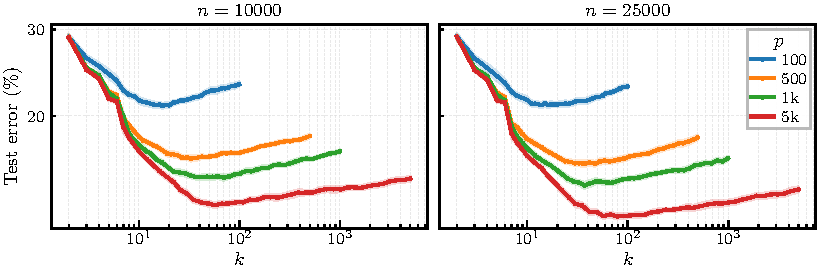
\includegraphics[width=\linewidth]{figs/error_vs_k_layers_2_ntrain_10000-25000_relu}
    \caption{
        Test error (\%) as a function of the number of retained features $k$ at the hidden layer, for a one-hidden-layer Neural LoFi with ReLU activation on CIFAR-10, for varying number of random projections $p$ and two training set sizes. The input and output layers are not reduced. The optimal $k$ increases with $p$, and larger $p$ consistently yields lower test error.
    }
    \label{2605:fig:sigmoid-one-layer}
\end{figure}

\begin{figure}
    \centering
    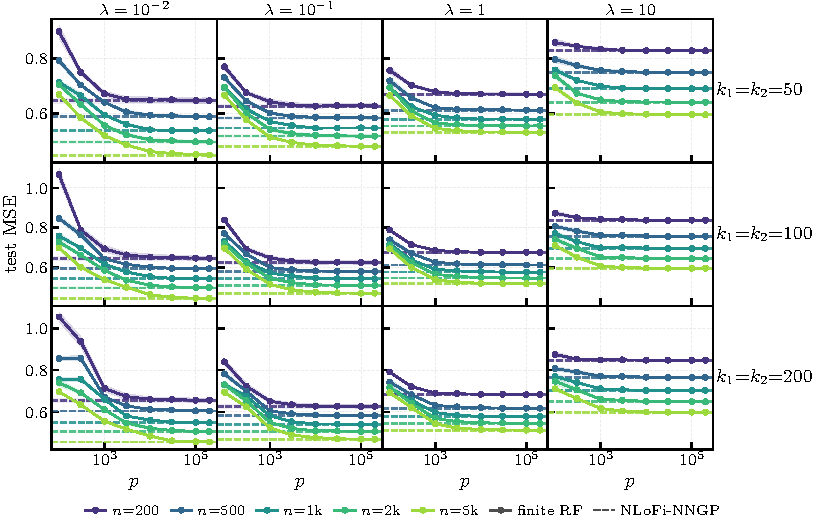
\includegraphics[width=\linewidth]{figs/plot_appendix_grid_c1}
    \caption{%
    Convergence of finite-width NLoFi to the NLoFi-NNGP limit as the hidden width $p$ grows.  Each panel shows the test MSE versus $p$ for four training-set sizes $n$. 
    Solid curves are finite-RF NLoFi; dashed horizontal lines mark the corresponding NLoFi-NNGP limits at the same $n$.  Rows vary the number of retained eigenfeatures per layer ($k_1 = k_2 \in \{50, 100, 200\}$); columns vary the ridge regularisation $\lambda$.
    Across all settings the finite-width curves converge from above to the kernel limit.%
    }  
    \label{2605:fig:nlofi-convergence}
\end{figure}


\subsection{Filtering of Features}

\Cref{2605:fig:sigmoid-one-layer} shows the test error as a function of $k$ for a single hidden layer, where only the intermediate representation is subject to Neural LoFi's feature selection. The curve structure mirrors the two-dimensional heatmaps of~\Cref{2605:fig:heatmaps}, now collapsed to a single axis. As $p$ increases the resulting test error improves and the optimal number of retained features $k^\star$ increases.
Crucially, selecting too few or too many features degrades performance, confirming that the U-shaped trade-off observed in \Cref{2605:fig:heatmaps}.


\subsection{Predicting the sample complexity for feature recovery}
\label{2605:app:feature-recovery}

% The variational analysis of Section~\ref{2605:sec:emergence-snr} predicts that
% the $k$-th eigenvector of the layer-$\ell$ signed covariance becomes
% recoverable when the population correlation $\rho_\ell^{(k)}$ exceeds the
% empirical noise floor $\tau_\ell^k(n)$, with the latter controlled by the
% residual effective dimension of the kernel induced by the previous layer.
% This is an asymptotic and abstract statement; whether the corresponding
% \emph{quantitative} prediction
% Eq.~\eqref{2605:eq:real-data-emergence-estimate} has any predictive content on
% real images is not obvious. 
% The bound underlying it relies on assumptions that are not satisfied by CIFAR-10
% features by design. 


The variational analysis of Section~\ref{2605:sec:emergence-snr} predicts
that the $k$-th eigenvector of the layer-$\ell$ signed covariance
becomes recoverable once the population correlation $\rho_\ell^{(k)}$
exceeds the empirical noise floor $\tau_\ell^k(n)$, with the latter
controlled by the residual effective dimension of the kernel induced by
the previous layer.  This is an asymptotic statement, and the
quantitative prediction
Eq.~\eqref{2605:eq:real-data-emergence-estimate} rests on assumptions that
CIFAR-10 features are not designed to satisfy.  The experiment in
Fig.~\ref{2605:fig:sample-complexity-pred} (and its convolutional analog
Fig.~\ref{2605:fig:sample-complexity-pred-conv}) is intended as a stress test
of the prediction in that regime.

% The experiment in
% Figure~\ref{2605:fig:sample-complexity-pred} in the main is intended as a stress test of the
% prediction in this regime. The experiment is also repeated on convolutional architecture, see Fig.\ref{2605:fig:sample-complexity-pred-conv}.


% We use the full binary CIFAR-10 training set ($N=60{,}000$ animals vs.\
% vehicles) as a population proxy: running Neural LoFi on this set yields
% stable reference eigenvectors $\{\hat{\bm v}_i^{(N)}\}_{i\ge 1}$ at the
% layer of interest. We then refit the same pipeline on random subsets of
% size $n\le N$, holding the random projections $\bm W_1,\bm W_2$ fixed
% across subsets, and record the index-aligned overlap
% $|\langle \hat{\bm v}_i^{(n)},\hat{\bm v}_i^{(N)}\rangle|^2$, averaged over
% $100$ independent dataset permutations. The predicted thresholds $n_\ell^k$ are obtained from the proxy at $n=N$ by the
% recursive procedure of App.~\ref{2605:app:effective-dimension}, and use no
% information from the smaller-$n$ runs.

% The predicted thresholds (dashed verticals) track the order and approximate
% scale of the empirical transitions across the six leading eigenvectors,
% which themselves are sharp on a logarithmic scale and proceed in order of
% decreasing $|\lambda_k|$, as in the BBP/EA picture of
% Section~\ref{2605:sec:emergence-snr}. 

% The bound underlying Eq.~\eqref{2605:eq:real-data-emergence-estimate} is
% qualitative and not tight, so the prediction should be read as the correct
% scaling of $n^k_\ell$ with the residual effective dimension and the
% spectral gap, rather than as an absolute threshold. Even at this level,
% however, the agreement is enough for
% Eq.~\eqref{2605:eq:real-data-emergence-estimate} to serve as a diagnostic: a
% single eigendecomposition on a reference set indicates the order of
% magnitude at which each eigendirection becomes extractable.

We use the full binary CIFAR-10 training set ($N=60{,}000$, animals
vs.\ vehicles) as a population proxy: running Neural LoFi on this set
yields stable reference eigenvectors $\{\hat{\bm v}_i^{(N)}\}_{i\ge 1}$
at the layer of interest.  We then refit the same pipeline on random
subsets of size $n\le N$, holding the random projections $\bm W_1,\bm
W_2$ fixed across subsets, and record the index-aligned overlap
$|\langle \hat{\bm v}_i^{(n)},\hat{\bm v}_i^{(N)}\rangle|^2$, averaged
over $100$ independent dataset permutations.  In the convolutional
figure we plot the eight overlaps after sorting them descending within
each draw, which is robust to the $|\lambda|$-ordering swaps that arise
when two leading eigenvalues of opposite sign have similar magnitude.  The predicted thresholds $n_\ell^k$
are obtained from the proxy at $n=N$ by the recursive procedure of
App.~\ref{2605:app:effective-dimension} and use no information from the
smaller-$n$ runs.

The predicted thresholds (dashed verticals) track the order and
approximate scale of the empirical transitions across the eight leading
eigenvectors, which themselves are sharp on a logarithmic scale and
saturate in the order predicted by the recursive effective-dimension
recipe — consistent with the BBP/EA picture of
Section~\ref{2605:sec:emergence-snr}.  The bound is qualitative and not
tight, so the prediction should be read as the correct scaling of
$n^k_\ell$ with the residual effective dimension and the spectral gap
rather than as an absolute threshold; even at this level, however, a
single eigendecomposition on a reference set is enough to indicate the
order of magnitude at which each eigendirection becomes extractable.

\begin{figure}
    \centering
    % \includegraphics[width=\linewidth]{overlap-gnn.png}
    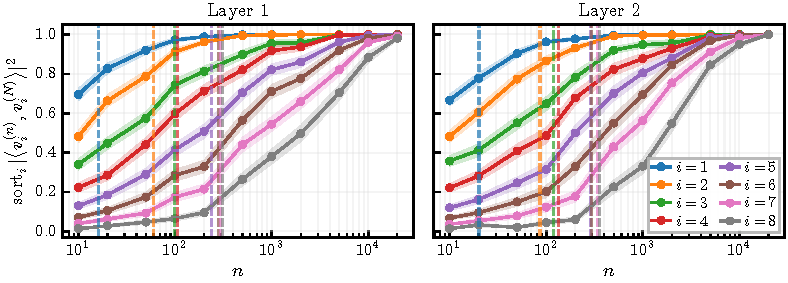
\includegraphics[width=\linewidth]{figs/paper_v1_fixedW0_100s_sortI_k1to8_two_panel}
    \caption{
    % \textbf{Predicting when individual features emerge on CIFAR-10 with convolutional networks.} This is the convolutional analog of 
    % Fig. \ref{2605:fig:sample-complexity-pred} in the main text.    
    % For a GNN  Neural LoFi model on the CIFAR-10 animal-vs.-vehicle task, we track the squared overlap
    % $|\langle v_i^{(n)},v_i^{(N)}\rangle|^2$
    % between eigenvectors estimated from \(n\) samples and large-sample reference eigenvectors.. Curves show mean \(\pm\) SEM over 100 random subsamples at fixed random features. Dashed vertical lines indicate the predicted emergence thresholds \(n_\ell^i\) from \eqref{2605:eq:lofi-emergence-threshold},\eqref{2605:eq:emergence_feature}
    % (see Eq.~\eqref{2605:eq:real-data-emergence-estimate} in Appendix). The sharp rise of each overlap near its predicted threshold shows that the effective-dimension criterion predicts when individual task-relevant directions become learnable.
    \textbf{Predicting when individual features emerge on CIFAR-10 with convolutional networks.} Convolutional analog of Fig.~\ref{2605:fig:sample-complexity-pred} in the main text.
    For a CNN Neural LoFi model on the CIFAR-10 animal-vs.-vehicle task (random feature matrices $\bm W_1, \bm W_2$ held fixed across subsamples), we track the squared overlap $|\langle v_i^{(n)},v_i^{(N)}\rangle|^2$ between eigenvectors estimated from $n$ samples and the large-sample reference eigenvectors at layer $1$ (Left) and $2$ (Right).  At each sample size we order the eight tracked overlaps from largest to smallest within each draw, so $i=1$ is the best-aligned axis at that $n$ and so on; curves show mean $\pm$ SEM over $100$ random subsamples.  Dashed verticals are the predicted emergence thresholds $n_\ell^k$ from \eqref{2605:eq:lofi-emergence-threshold},\eqref{2605:eq:emergence_feature},
    sorted ascending and color-matched to the curves (see
    Eq.~\eqref{2605:eq:real-data-emergence-estimate} in the Appendix).   The sharp rise of each curve near its predicted threshold shows that the effective-dimension criterion predicts the order and approximate scale at which successive task-relevant directions become learnable.
    }
    \label{2605:fig:sample-complexity-pred-conv}
\end{figure}



\subsection{Spectrum of the signed covariance}
The core of LoFi is the spectral decomposition of the signed covariance operator, thus it is crucial to understand the structure of its spectrum. 

We analyze the eigenvalue spectra learned by ridge spectral networks on a binary CIFAR-10 classification task (animal vs. vehicle). The architecture comprises two convolutional layers with $p=512$ channels, each followed by $2\times 2$ max pooling and $L_2$ normalization of the features—concluding with a fully-connected layer of $p=512$ units. All layers are trained using signed-covariance eigendecomposition with eigenvalue-based feature selection (ridge spectral training). We evaluate the model across a range of training set sizes ($n \in \{200, 500, 2000, 50000\}$) while maintaining a fixed network architecture. The grid plots in \Cref{2605:fig:eigenvalues-histogram} illustrate the full eigenvalue spectrum for each layer, utilizing a symlog $x$-axis to resolve both fine-grained and large-magnitude spectral components. The top five eigenvalues per layer are highlighted with red triangles, revealing how the spectral structure evolves with data scale and illustrating the relative importance of dominant versus distributed features across the network depth.
\begin{figure}
    \centering
    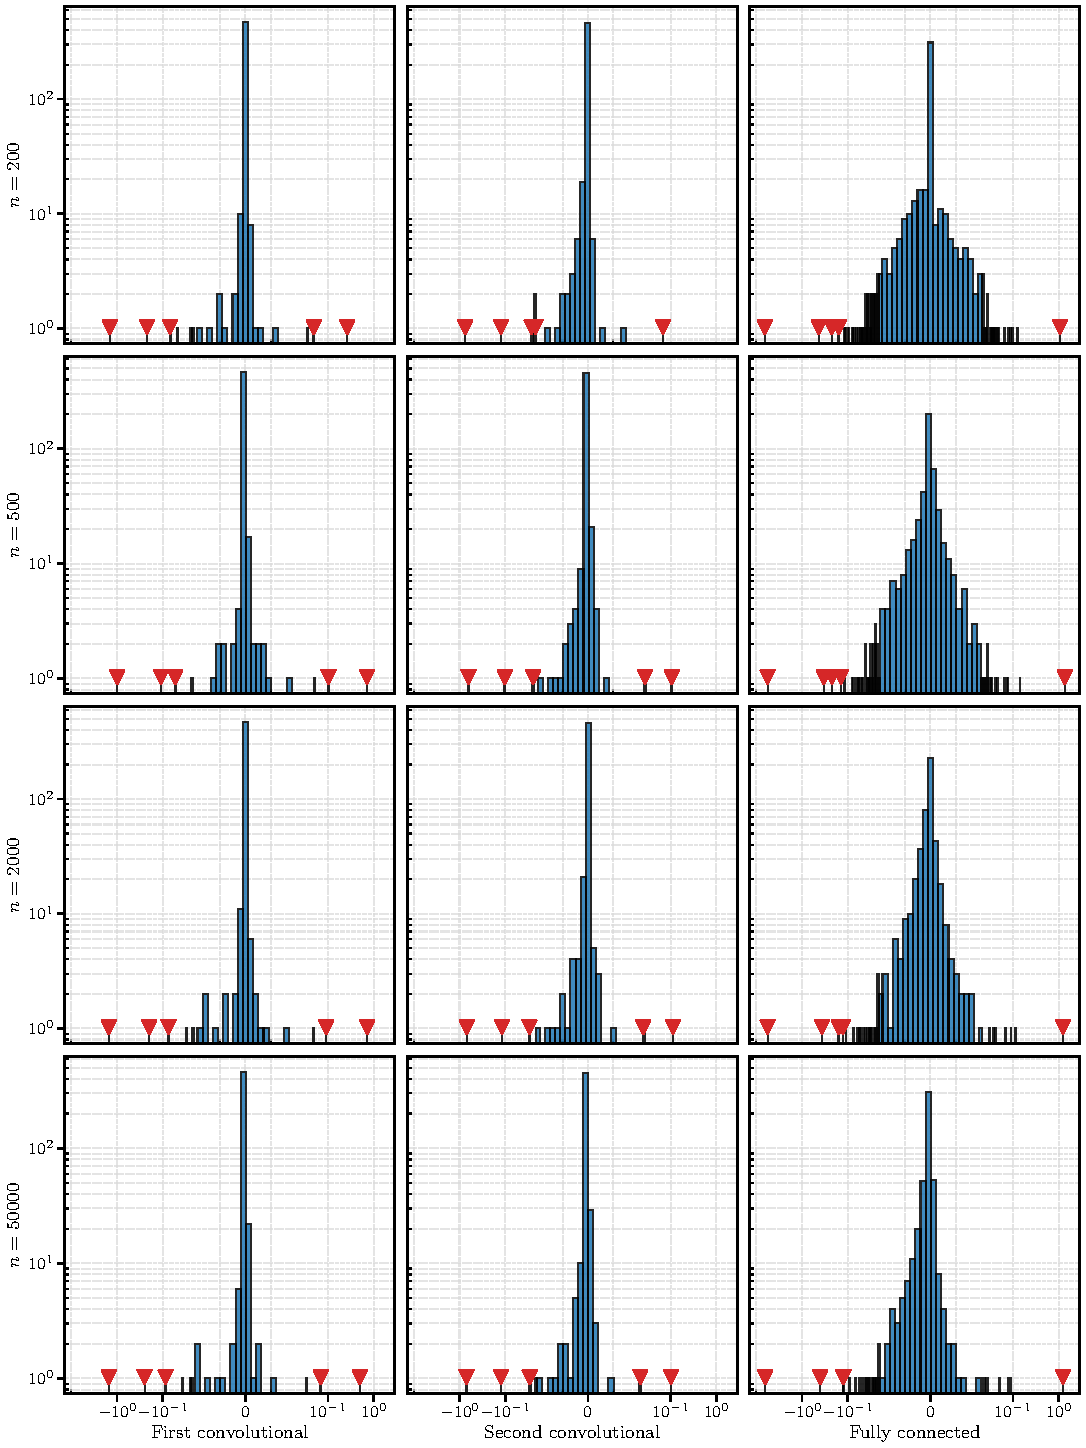
\includegraphics[width=0.94\linewidth]{figs/eigvals_hist_grid}
    \caption{\textbf{Spectral Distribution:} Histograms of eigenvalues across network layers (columns) and dataset sizes (rows). Red markers indicate the five most dominant eigenvalues. The symlog scale reveals the emergence of spectral structure and the separation of lead features from the bulk distribution as $n$ grows. The random feature dimension in this experiment is $p=512$ for all layers.}
    \label{2605:fig:eigenvalues-histogram}
\end{figure}


\subsection{Feature Visualization}

\begin{figure}
    \centering
    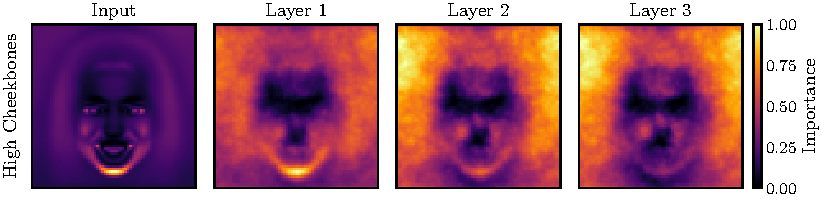
\includegraphics[width=\linewidth]{figs/high_cheekbones_ntrain200000_P50000_layers3_keep100-50-20_relu_seed0_signed_cov}\\
    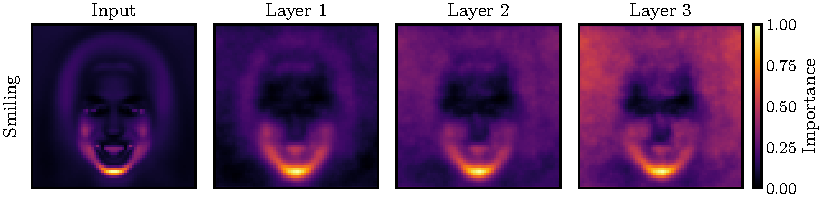
\includegraphics[width=\linewidth]{figs/smiling_ntrain200000_P50000_layers3_keep100-50-20_relu_seed0_signed_cov}
    \caption{
    Layer-wise feature importance $\bar{I}^{(\ell)}$ (\cref{2605:eq:importance-layer}) on CelebA \cite{liu2015deep} for two binary 
    attributes. \textit{(Top, High Cheekbones)} Importance concentrates 
    progressively on the cheekbone region across layers, while the chin area, 
    salient at the input, is progressively suppressed in deeper layers. 
    \textit{(Bottom, Smiling)} Importance remains focused on the mouth and jaw 
    region throughout all layers, reflecting that the discriminative signal for 
    this attribute is preserved and not discarded by Neural LoFi's feature 
    selection. This contrast illustrates that the retained features are 
    task-dependent and geometrically meaningful.
    }
    \label{2605:fig:celeba-feature-importance}
\end{figure}


\paragraph{Input importance} To probe which input pixels drive the activation along $v_k^{(\ell)}$, we
back-propagate through the random features and accumulate the absolute
Jacobian--vector product over the training set,
\begin{equation}
  I_k^{(\ell)}(d)  =  \frac{1}{N}\sum_{i=1}^{N}
  \left| \frac{\partial}{\partial x_{i,d}}  \left( v_k^{(\ell) \top} \phi_\ell(x_i) \right) \right|
   =  \frac{1}{N}\sum_{i=1}^{N} \left| J_\ell(x_i)^{ \top} v_k^{(\ell)} \right|_d,
  \label{2605:eq:importance_per_k}
\end{equation}
where $J_\ell(x) = \partial \phi_\ell(x)/\partial x \in \mathbb{R}^{P\times D}$.
The raw map $I_k^{(\ell)}$ is convolved with an isotropic Fourier low-pass
filter $\smash{m(f) = (1 + \|f\|/f_0)^{-\alpha}}$ to suppress
high-frequency noise inherited from the random projections. For the input layer ($\ell = 0$) the Jacobian collapses to the identity and~\eqref{2605:eq:importance_per_k} reduces to
$I_k^{(0)}(d) = \bigl(v_k^{(0)}\bigr)_d^{2}$.

Different eigenvectors carry very different amounts of label signal. Rather than
treating them uniformly, we aggregate the $K_\ell$ retained per-$k$ importance
maps with weights given by the absolute signed-covariance eigenvalues,
\begin{equation}\label{2605:eq:importance-layer}
  \bar{I}^{(\ell)}(d)  = \frac{\sum_{k=0}^{K_\ell-1} |\lambda_k^{(\ell)}|  I_k^{(\ell)}(d)}{\sum_{k=0}^{K_\ell-1} |\lambda_k^{(\ell)}|}.
\end{equation}
This emphasises directions that most strongly co-vary with the target while
preserving the spatial information carried by the lower-ranked, but still
label-aligned, eigenvectors.

In~\Cref{2605:fig:celeba-feature-importance} each panel shows $\bar{I}^{(\ell)}$ reshaped to the $64 \times 64$ image grid and averaged over the three colour channels. We min--max rescale each panel independently to $[0,1]$. 
The shared colorbar reports this per-panel normalised intensity. The vertical label on the leftmost panel names the binary CelebA attribute used as $y$.

\paragraph{Filter and activations for CNNs} In Section~\ref{2605:sec:real-data} we have already discussed the filters and activations learned by LoFi for CNNs. Here we provide additional visualizations of these filters and activations, for different layers and training set sizes.
\begin{figure}
    \centering
    \begin{minipage}{0.3\linewidth}
    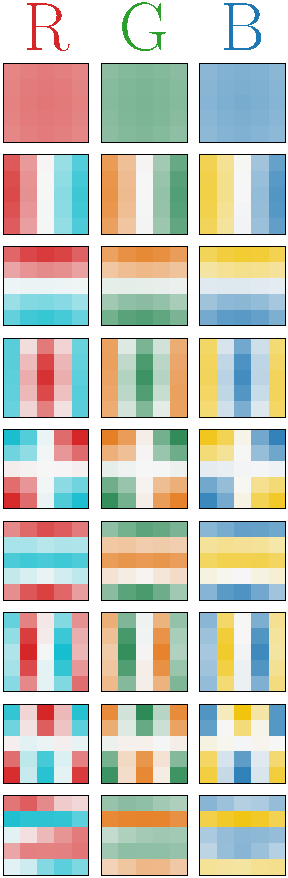
\includegraphics[width=0.8\linewidth]{figs/celeba_filters}
    \end{minipage}
    
    \begin{minipage}{0.6\linewidth}
        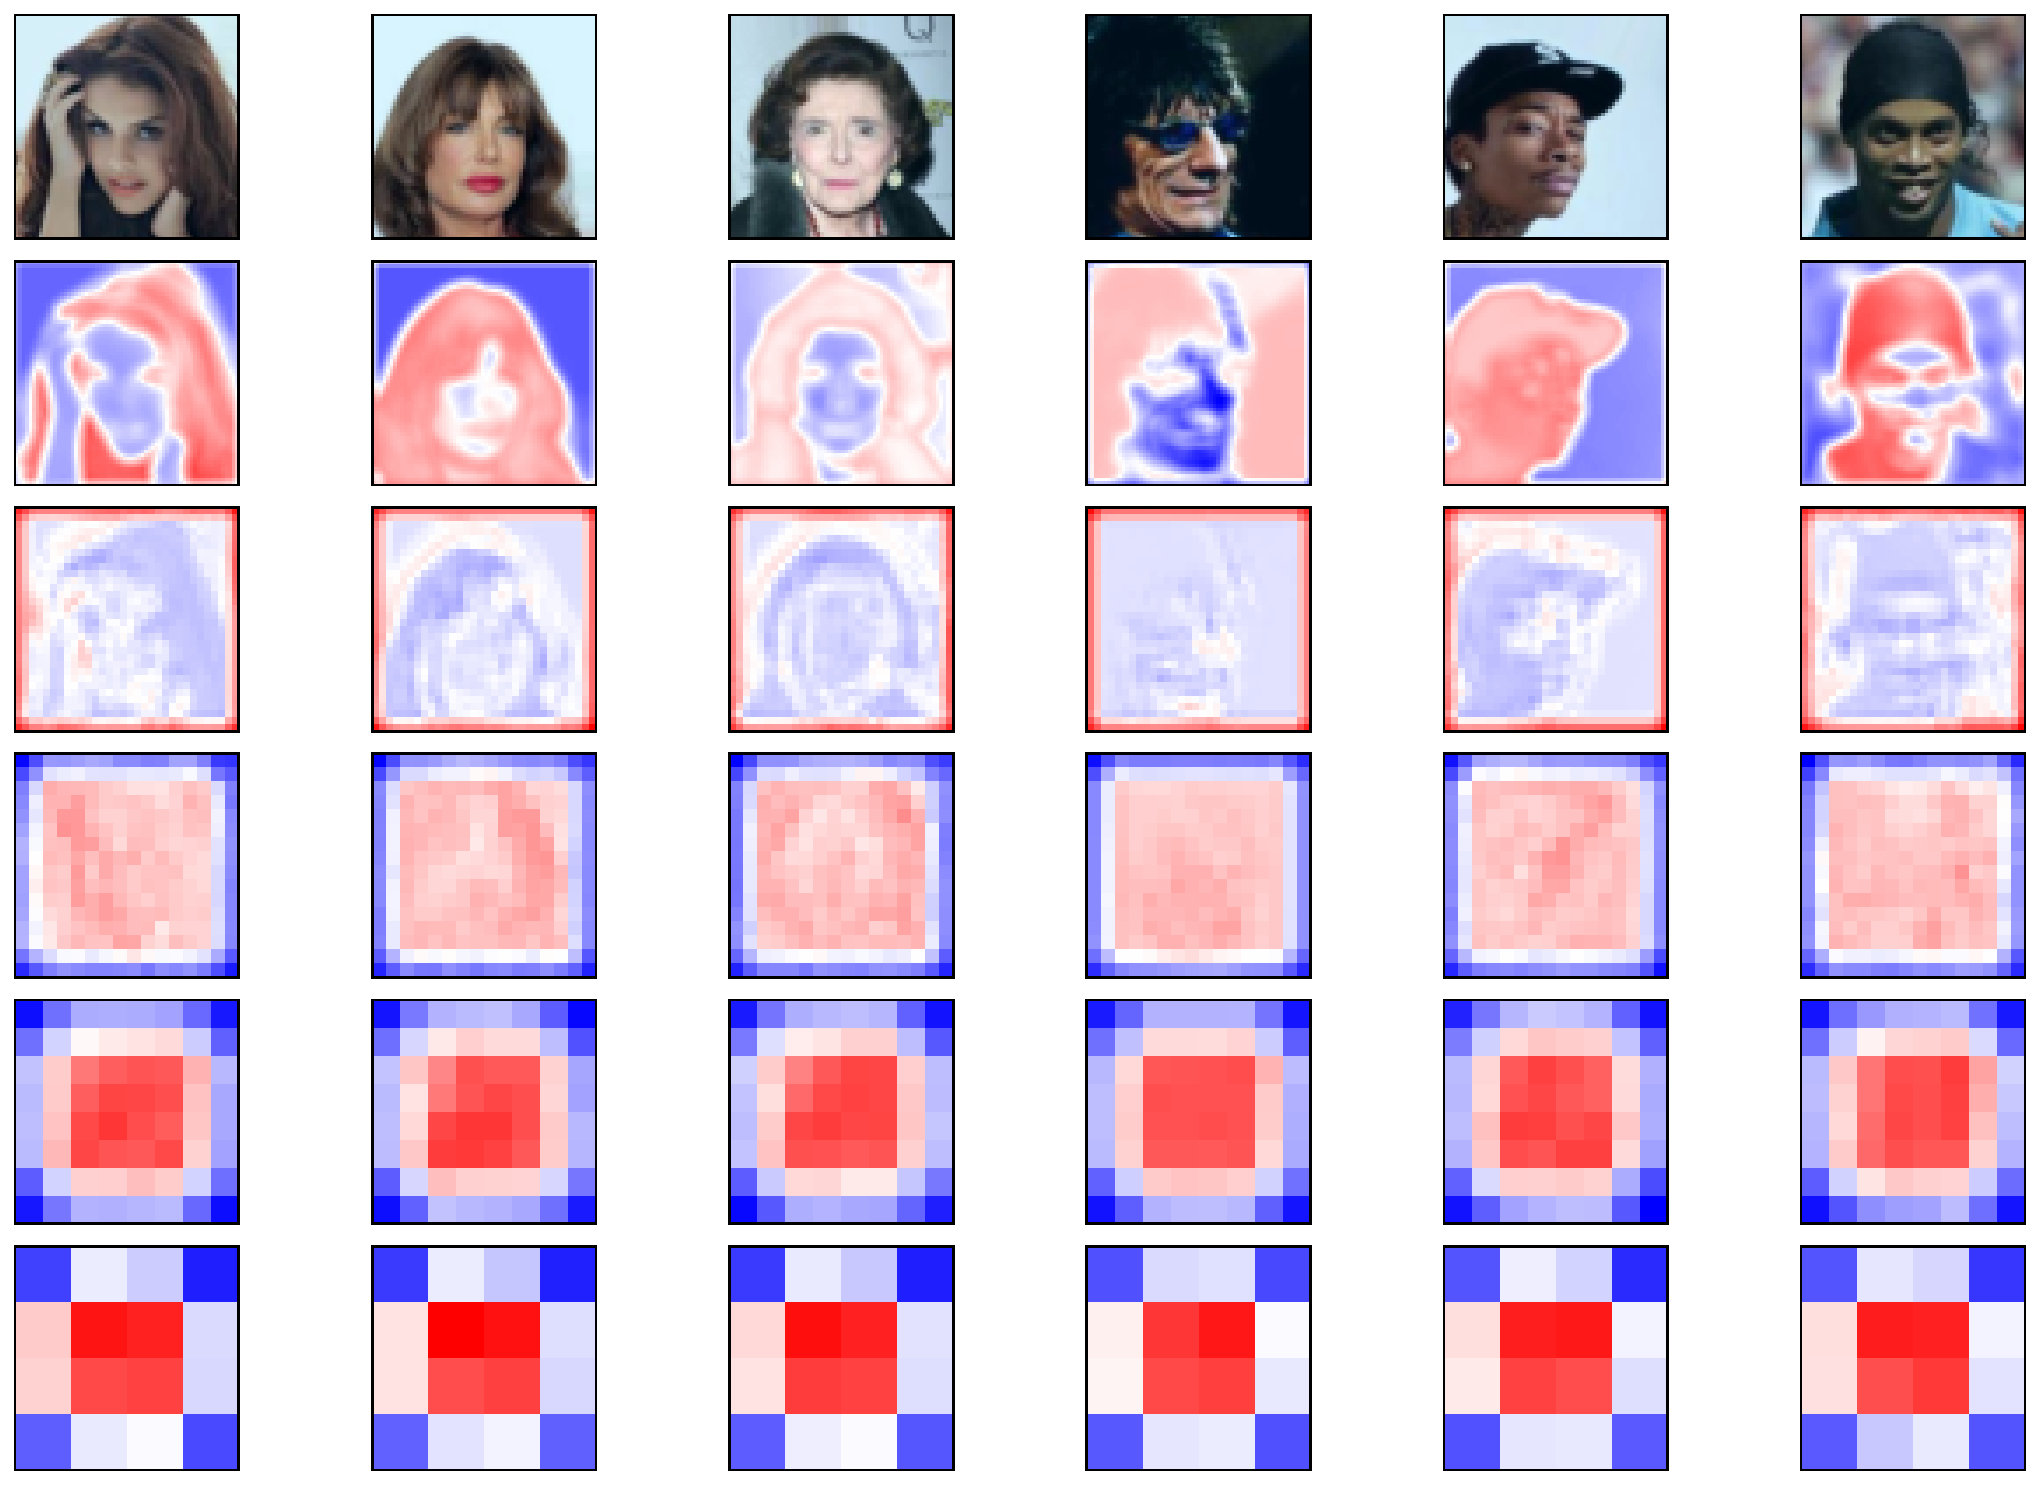
\includegraphics[width=0.8\linewidth]{figs/rank_01_definitive_activations}
        \begin{center}activation of top eigenvector \end{center}
        

        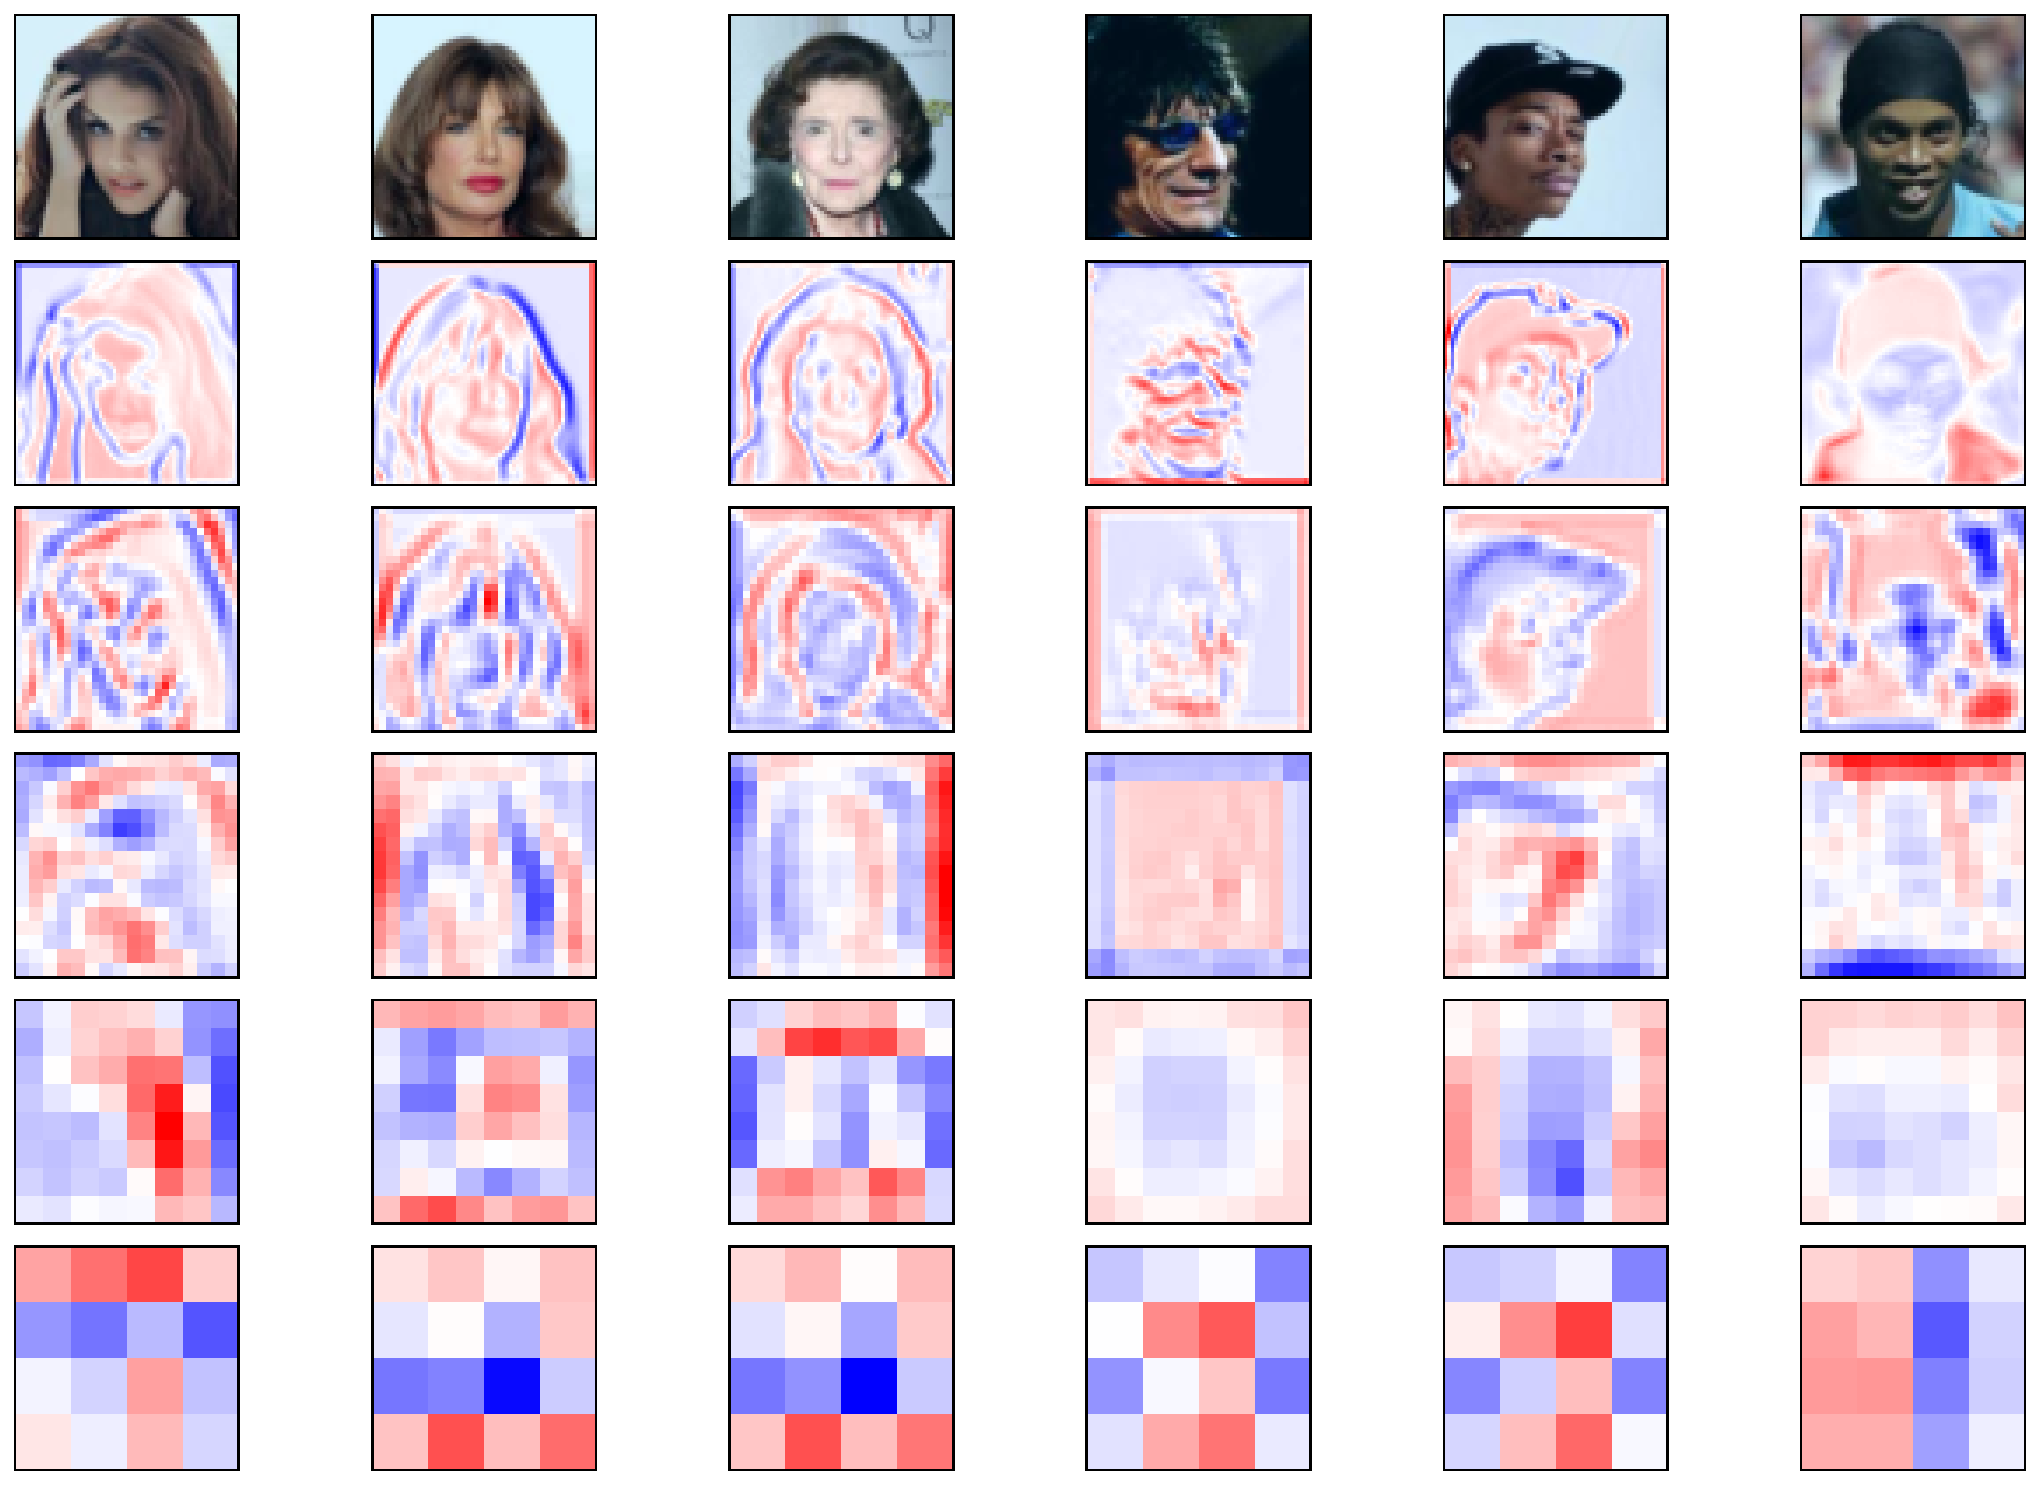
\includegraphics[width=0.85\linewidth]{figs/rank_07_definitive_activations}
        \begin{center}activation of 7th eigenvector \end{center}
    \end{minipage}
    \caption{\textbf{Filters and activations for CNNs.} We train a 6 convolutional + 1 fully connected layer neural network on CelebA \cite{liu2015deep} for binary classification of the "Gender" attribute, using Neural LoFi with signed-covariance eigendecomposition and eigenvalue-based feature selection. \textit{(Left)} The $5\times5$ first-layer filters learned by Neural LoFi, visualized as RGB images. \textit{(Right)} The activations of the top-ranked (1st) and mid-ranked (7th) eigenvectors at each convolutional layer (lower rows are deeper), for 6 images of the test set.}
    \label{2605:fig:additional-cnn-feature-visualizations}
\end{figure}
In Figure~\ref{2605:fig:additional-cnn-feature-visualizations} we show the first-layer filters learned by LoFi, as well as the activations of the top-ranked and mid-ranked eigenvectors at each convolutional layer. Despite being larger than the filters learned on CIFAR-10 (Figure~\ref{2605:fig:cnn-filter-activations}), the filters learned on CelebA are still interpretable as edge detectors, with a variety of orientations and frequencies. It is interesting to compare the features learned by different eigenvectors: the top eigenvector tends to be a brightness filter and converges to the same representation when going deeper. The mid-ranked eigenvector, instead, learns more complex features even at the first layer, obtaining a self-evident representation of the sample after the last convolutional layer.
